\documentclass[border=10pt]{standalone}
\usepackage{tikz}
\usetikzlibrary{arrows.meta, shapes, calc}

\renewcommand{\Large}{\small}\begin{document}

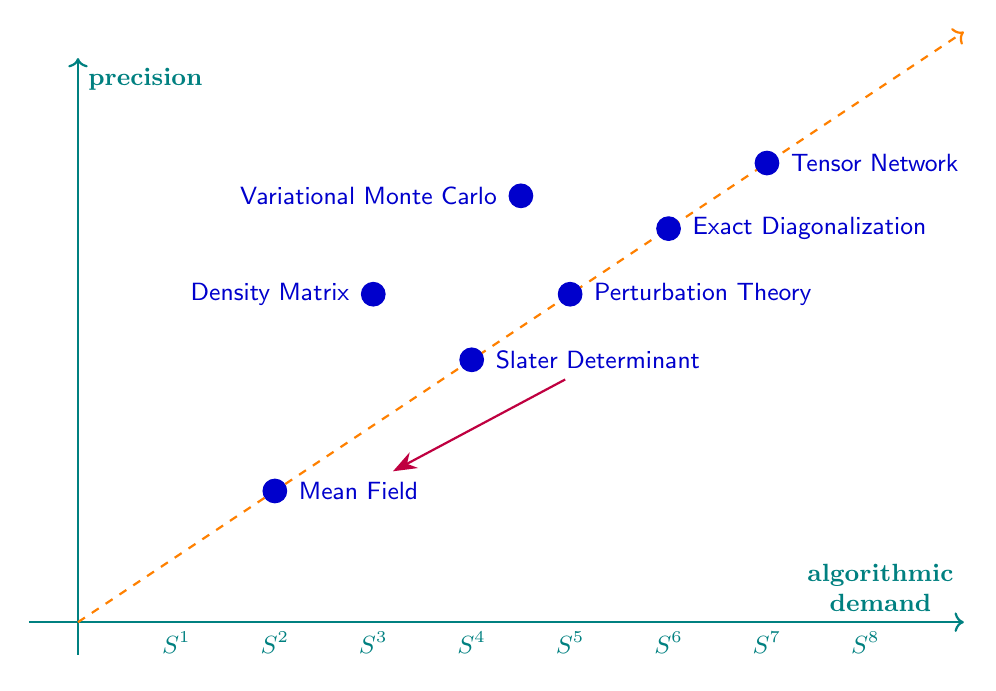
\begin{tikzpicture}[x=1.25cm,y=0.833cm]
    % Axes
    \draw[->, thick, teal] (-0.5,0) -- (9,0) node[above left, align=center, font=\bfseries\Large] {algorithmic\\demand};
    \draw[->, thick, teal] (0,-0.5) -- (0,8.6) node[below right, font=\bfseries\Large] {precision};
    
    % Grid
    \foreach \x in {1,...,8} \node[below, teal, font=\Large] at (\x,0) {$S^\x$};
    
    % Lines
    \draw[->, dashed, thick, orange] (0,0) -- (9,9);
    \draw[thick, purple, -{Stealth[length=3mm]}] (4.95,3.7) -- (3.2,2.3);
    
    % Points and labels
    \filldraw[blue!80!black] (4.5,6.5) ellipse (0.12 and 0.18) node[left=1.2ex, font=\sffamily\Large] {Variational Monte Carlo};
    \filldraw[blue!80!black] (3,5) ellipse (0.12 and 0.18) node[left=1.2ex, font=\sffamily\Large] {Density Matrix};
    \filldraw[blue!80!black] (2,2) ellipse (0.12 and 0.18) node[right=1.2ex, font=\sffamily\Large] {Mean Field};
    \filldraw[blue!80!black] (4,4) ellipse (0.12 and 0.18) node[right=1.2ex, font=\sffamily\Large] {Slater Determinant};
    \filldraw[blue!80!black] (5,5) ellipse (0.12 and 0.18) node[right=1.2ex, font=\sffamily\Large] {Perturbation Theory};
    \filldraw[blue!80!black] (6,6) ellipse (0.12 and 0.18) node[right=1.2ex, font=\sffamily\Large] {Exact Diagonalization};
    \filldraw[blue!80!black] (7,7) ellipse (0.12 and 0.18) node[right=1.2ex, font=\sffamily\Large] {Tensor Network};
    
\end{tikzpicture}

\end{document}
